

%===================================
%===================================
\section{Pruebas}
\label{sec:Pruebas}

En esta sección se presentan las pruebas realizadas para validar el funcionamiento del sistema desarrollado. Se describen los casos de prueba, los resultados obtenidos y las conclusiones derivadas de dichas pruebas. Se hace la comparación entre los resultados de las dos máquinas descritas anteriormente, con el fin de evaluar el rendimiento del sistema en diferentes entornos.

Para las optimizaciones por compilador se usaron las banderas \texttt{-O3 -Wall -march=native -funroll-loops -flto -ffast-math -fomit-frame-pointer}.

El signigicado de cada bandera es el siguiente:
\begin{itemize}
   \item \textbf{-O3:} Esta bandera habilita un nivel de optimización agresivo, permitiendo al compilador aplicar una amplia gama de técnicas para mejorar el rendimiento del código.
   \item \textbf{-Wall:} Activa la mayoría de las advertencias del compilador, lo que ayuda a identificar posibles problemas en el código que podrían afectar su rendimiento o funcionalidad.
   \item \textbf{-march=native:} Permite al compilador generar código optimizado para la arquitectura específica del procesador en el que se está compilando, aprovechando las características y capacidades de hardware disponibles.
   \item \textbf{-funroll-loops:} Habilita el desenrollado de bucles, lo que puede mejorar el rendimiento al reducir la sobrecarga de control de bucle y aumentar la paralelización de las instrucciones.
   \item \textbf{-flto:} Habilita la optimización a nivel de enlace, lo que permite al compilador realizar optimizaciones globales en todo el programa, incluso entre diferentes archivos de código fuente.
   \item \textbf{-ffast-math:} Permite al compilador realizar optimizaciones agresivas en operaciones matemáticas, lo que puede mejorar el rendimiento a costa de la precisión en algunos casos como la evaluación de funciones trigonométricas.
   \item \textbf{-fomit-frame-pointer:} Indica al compilador que no utilice un puntero de marco para las funciones, es decir, que no cree un marco de pila para cada función, lo que puede mejorar el rendimiento al reducir la cantidad de instrucciones necesarias para gestionar la pila de llamadas.
\end{itemize}


%================================
\subsection{Ejecución del algoritmo secuencial}
\label{sec:Ejecución del algoritmo secuencial}

Se hizo la ejecución del algoritmo secuencial en una de las maquinas \texttt{m7i-flex.large} para mantener la validez del experimento. Para la ejecución de este algoritmo se hizo la compilación usando las flags antes mencionadas.

\begin{table}[H]
   \centering
   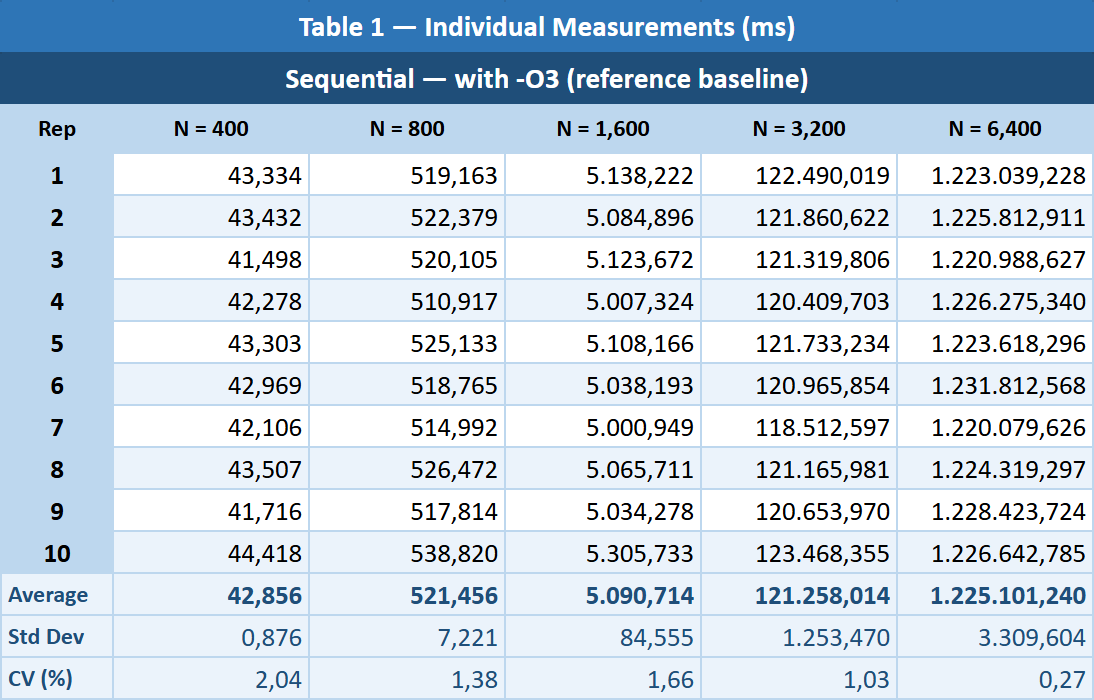
\includegraphics[width=1\textwidth]{images/tables/time_secuencial.png}
   \caption{Tiempo de ejecución del algotimo secuencial}
\end{table}


%================================
\subsection{Ejecución de la implementación con MPI}
\label{sec:Ejecución de la implementación con MPI}

\begin{table}[H]
   \centering
   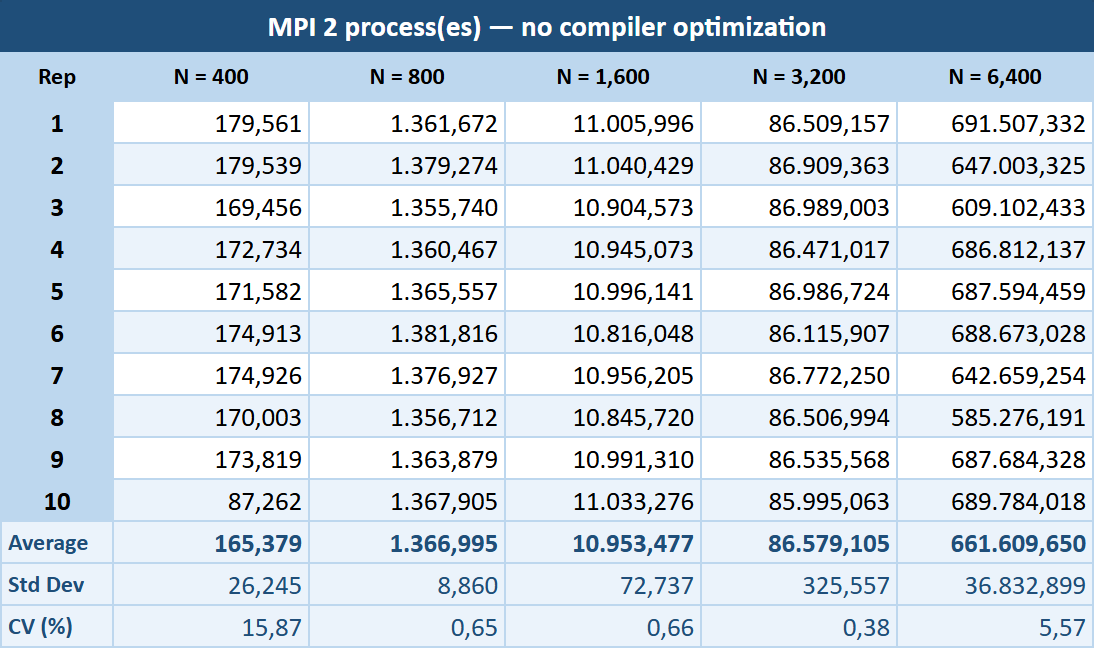
\includegraphics[width=1\textwidth]{images/tables/time_mpi_2_noopt.png}
   \caption{Tiempo de ejecución de la implementación con MPI con 2 procesos}
\end{table}

\begin{table}[H]
   \centering
   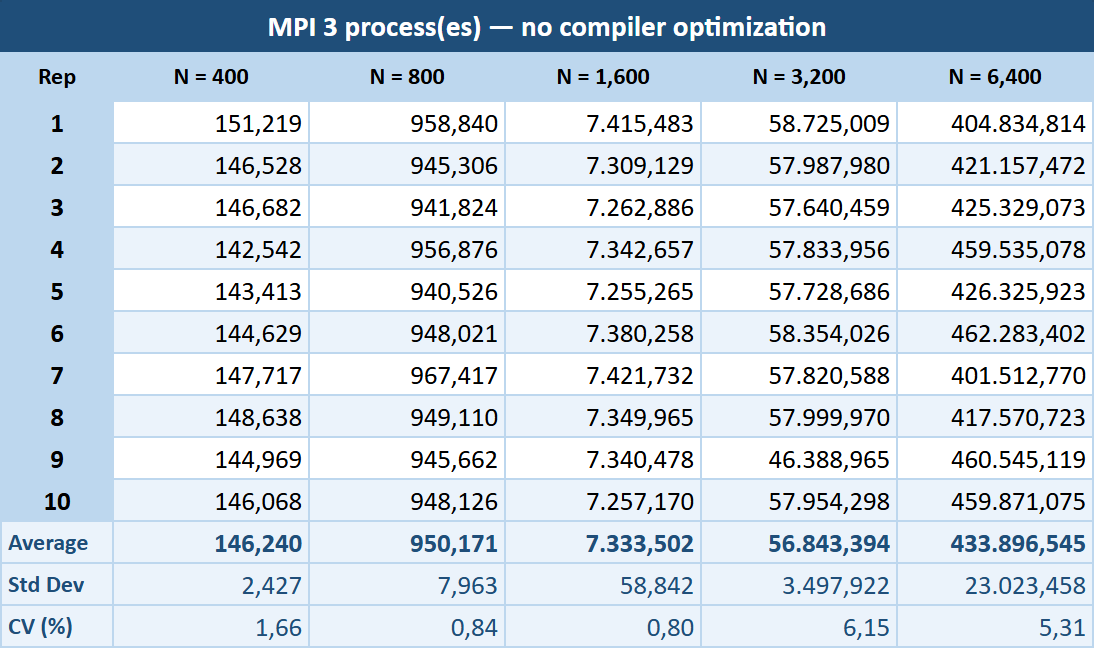
\includegraphics[width=1\textwidth]{images/tables/time_mpi_3_noopt.png}
   \caption{Tiempo de ejecución de la implementación con MPI con 3 procesos}
\end{table}

\begin{table}[H]
   \centering
   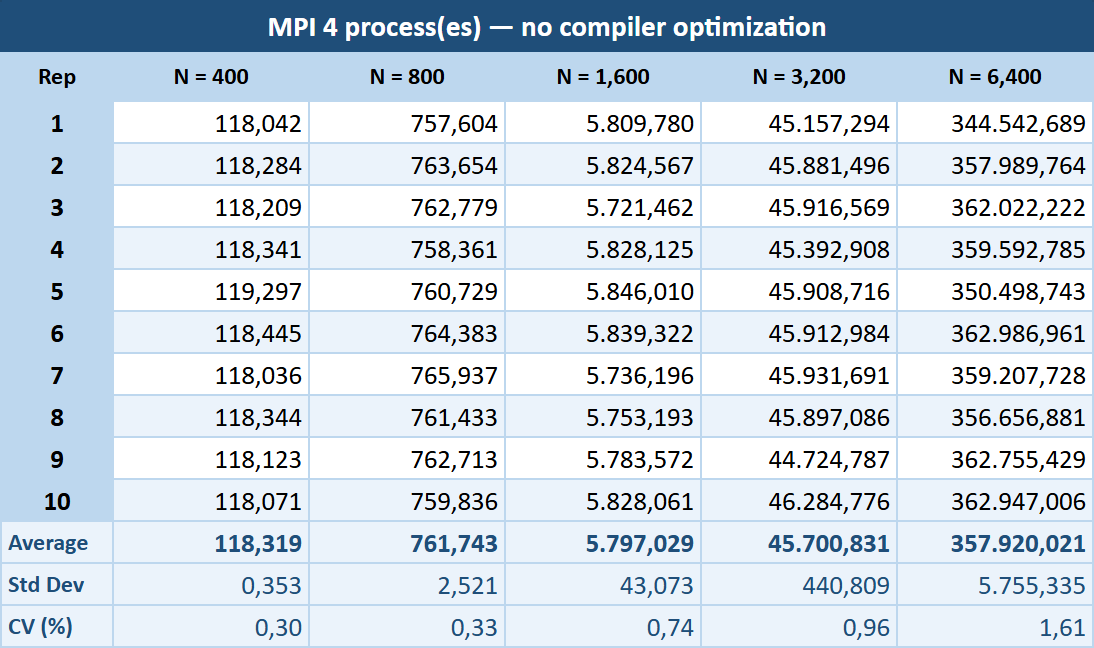
\includegraphics[width=1\textwidth]{images/tables/time_mpi_4_noopt.png}
   \caption{Tiempo de ejecución de la implementación con MPI con 4 procesos}
\end{table}


\subsubsection{Speedup}
\label{sec:Speedup}

\begin{table}[H]
   \centering
   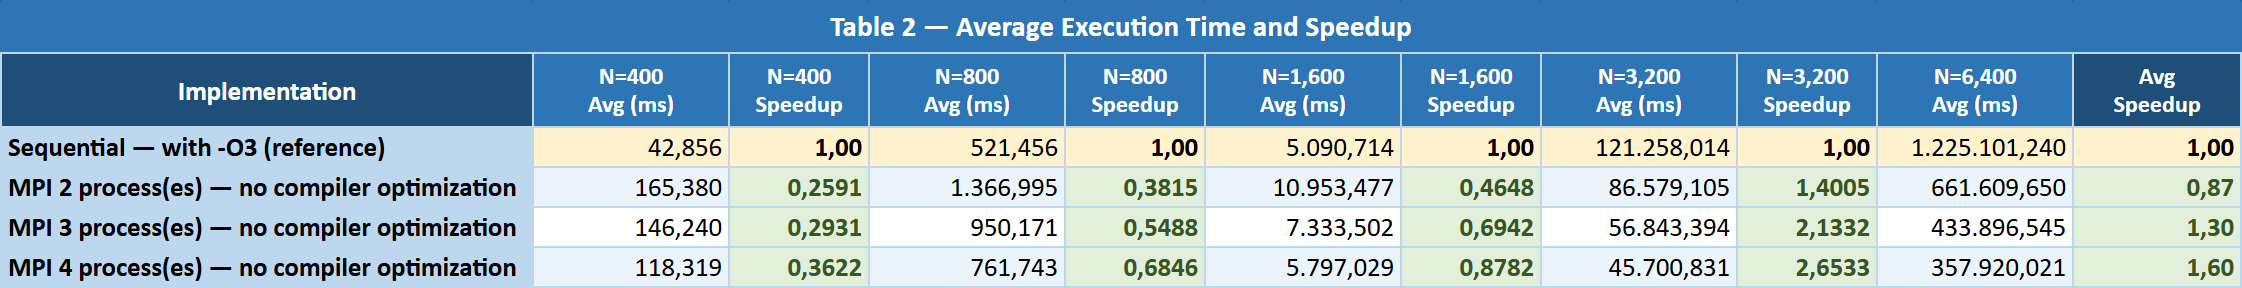
\includegraphics[width=1\textwidth]{images/tables/speedup_noopt.png}
   \caption{Tabla del speedup del la implementación con MPI sin optimizaciones}
\end{table}

\begin{figure}[H]
   \centering
   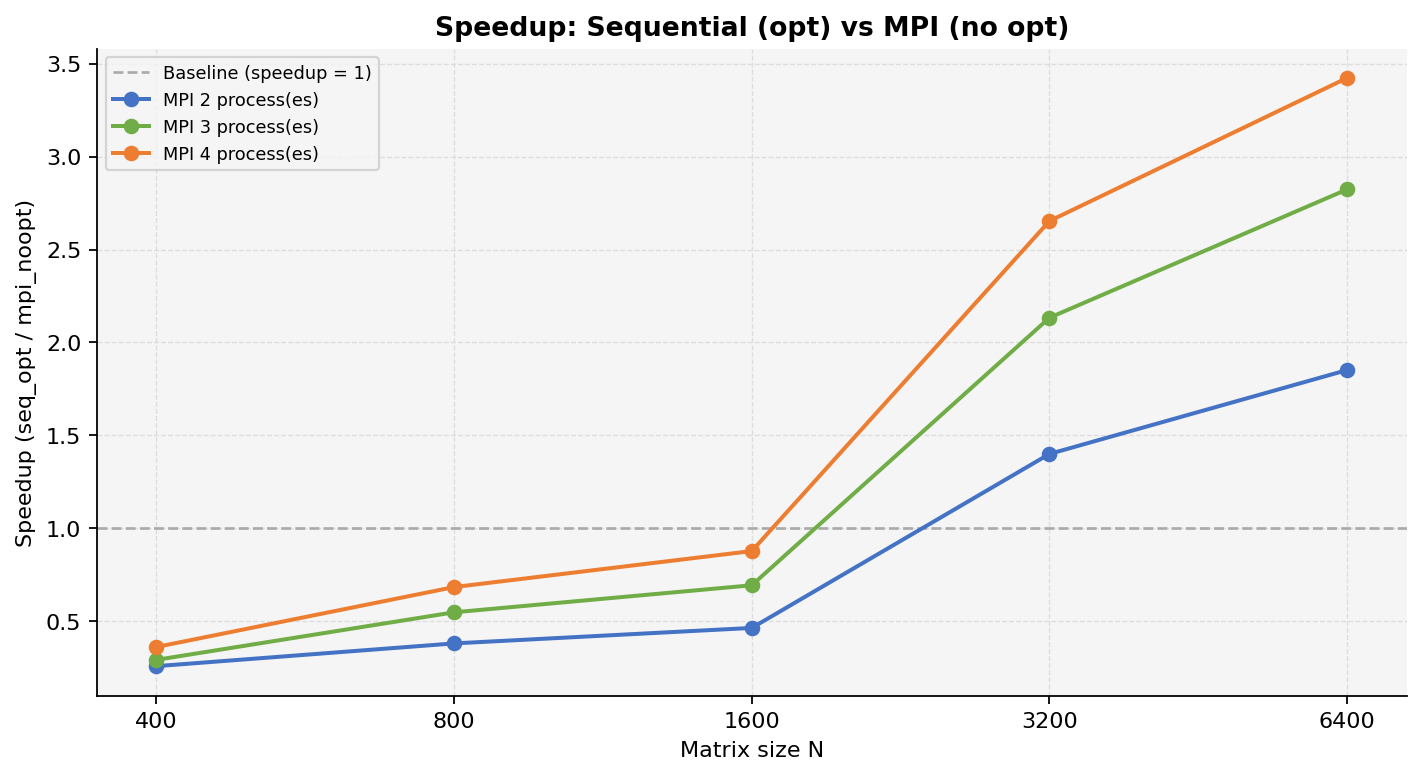
\includegraphics[width=1\textwidth]{images/charts/speedup_seq_vs_mpi_noopt.png}
   \caption{Speedup del la implementación con MPI sin optimizaciones}
\end{figure}



%================================
\subsection{Ejecución de la implementación con MPI con optimización por compilador}
\label{sec:Ejecución de la implementación con MPI con optimización por compilador}

\begin{table}[H]
   \centering
   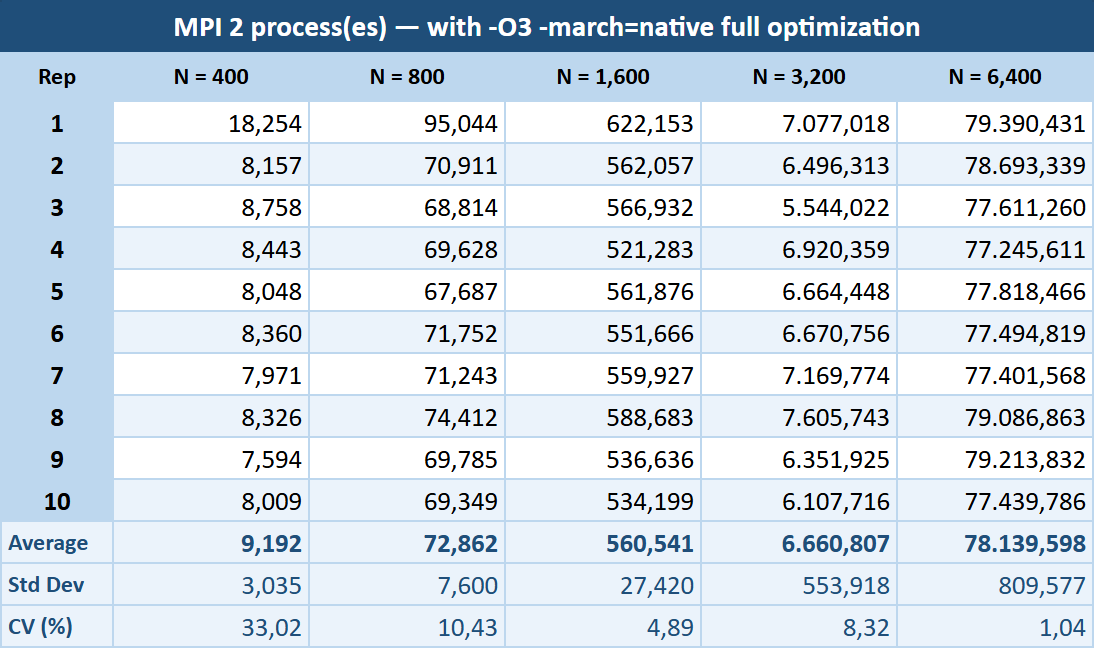
\includegraphics[width=1\textwidth]{images/tables/time_mpi_2_opt.png}
   \caption{Tiempo de ejecución de la implementación con MPI con optimizaciones con 2 procesos}
\end{table}

\begin{table}[H]
   \centering
   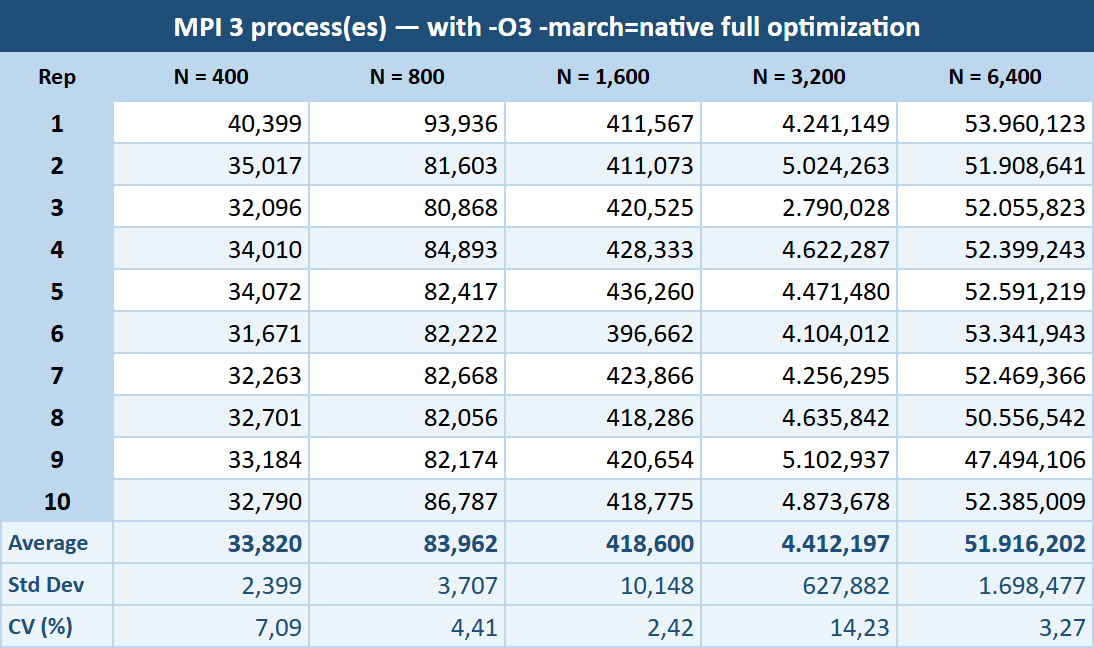
\includegraphics[width=1\textwidth]{images/tables/time_mpi_3_opt.png}
   \caption{Tiempo de ejecución de la implementación con MPI con optimizaciones con 3 procesos}
\end{table}

\begin{table}[H]
   \centering
   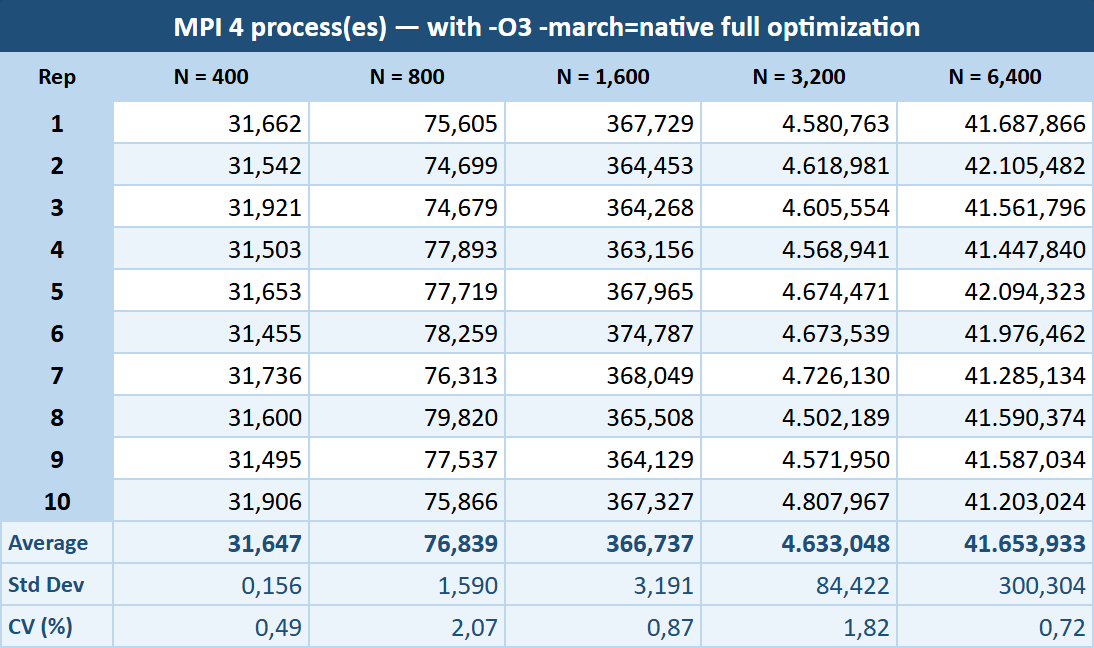
\includegraphics[width=1\textwidth]{images/tables/time_mpi_4_opt.png}
   \caption{Tiempo de ejecución de la implementación con MPI con optimizaciones con 4 procesos}
\end{table}


\subsubsection{Speedup}
\label{sec:Speedup opt}

\begin{table}[H]
   \centering
   
\includegraphics[width=1\textwidth]{images/tables/speedup_opt.png}
   \caption{Tabla del speedup del la implementación con MPI con optimizaciones}
\end{table}

\begin{figure}[H]
   \centering
   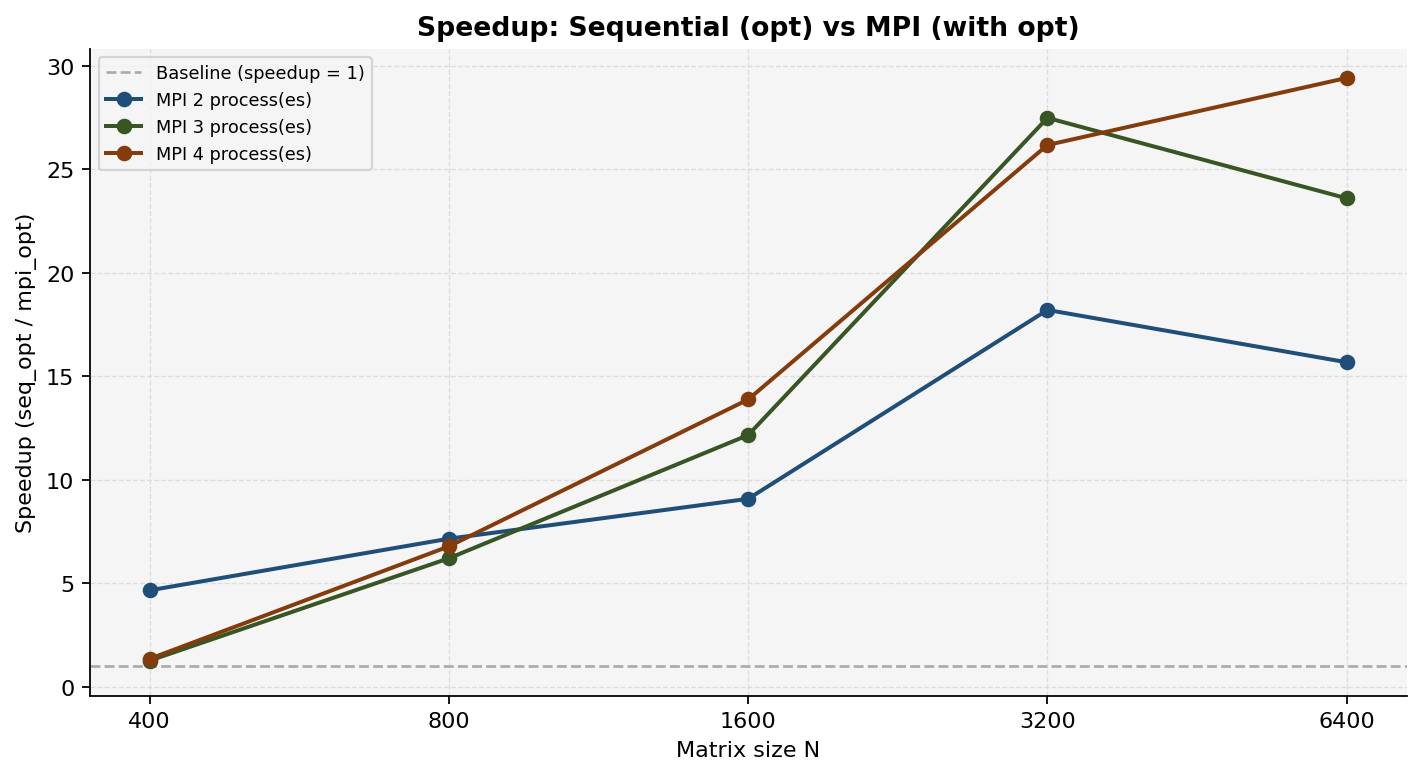
\includegraphics[width=1\textwidth]{images/charts/speedup_seq_vs_mpi_opt.png}
   \caption{Speedup del la implementación con MPI con optimizaciones}
\end{figure}